\chapter{Experimenty}

Cílem závěrečné kapitoly je ověřit vlastnosti implementovanách agentů pomocí experimentů a zhodnotit kvalitu natrénované
neuronové sítě. Nejprve je popsáno prostředí, v němž se experimenty konaly, následně je popsán turnaj implementovaných
agentů a jejich porovnání. Na závěr je pak diskutována kvalita natrénované neuronové sítě a porovnání botů mezi sebou
a proti lidskému hráči.

\section{Experimentální prostředí}

\subsection{Hardwarová a Softwarová konfigurace}

Experimenty byly prováděny na osobním počítači s procesorem Intel Core i7-14700KF, grafickou kartou NVIDIA GeForce RTX 4060 Ti a 32 GB operační paměti.
Experimenty kvality botů probíhaly zejména v prostředí napsaném v jazyce Python, v jazyce C\# je pouze graifcká aplikace.

Všechny experimenty byly provedeny nad stejnámi pravidly a stejnou implementací herního prostředí. Díky tomu jsou
rozdíly mezi jednotlivými agenty založeny čistě na jejich algoritmech. Více implementačních detailů v repozitáři~\cite{logix_gitlab}.

\subsection{Nastavení experimentů}

Pro porovnání agentů byl vytvořen turnajový skript. Každá dvojice agentů odehrála proti sobě 50 partií. Aby se eliminovala
výhoda prvního tahu, tak se agenti po každé partii střídají v počátečním tahu. Maximální délka hry je nastavena na 50 tahů,
delší hry z praxe moc neexistují. Po každé odehrané partii byly ukládány výsledky turnaje, což umožnilo turnaj kdykoliv
přerušit a znovu spustit bez ztráty odehraných partií.

V turnaji bylo porovnáno 5 agentů. Jednalo se o agenty popsané v sekci~\ref{sec:agents}: náhodného agenta, heuristického agenta,
agenta využívající minimax s alfa-beta ořezáváním a dvě varianty MCTS algoritmus. Ty se lišily použítím verze neuronové sítě, 
přičemž obě využívaly stejnou hloubku prohledávání.

\section{Porovnání herních agentů}

\subsection{Metodika}

Cílem experimentu bylo porovnat sílu všech implementovaných herních agentů při vzájemných partiích. Každý agent odehrál sérii 50 partií 
proti všem ostatním agentům. 

V turnaji bylo porovnáváno pět různých agentů představujících odlišné přístupy k rozhodování. Přehled použitých agentů je uveden v tabulce~\ref{tab:agents}.

\begin{table}[h]
\centering
\caption{Přehled porovnávaných agentů.}
\label{tab:agents}
\begin{tabular}{lll}
\toprule
Agent & Algoritmus & Parametry \\
\midrule
Random & Náhodný výběr tahu & -- \\
Heuristic & Ručně navržená heuristika & max\_safety\_checks = 10 \\
AlphaBeta & Minimax + alfa-beta & hloubka = 3 \\
MCTS-old & MCTS + neuronová síť & 100 simulací \\
MCTS-new & MCTS + neuronová síť & 100 simulací \\
\bottomrule
\end{tabular}
\end{table}

Za vítězství v partii získal agent jeden bod, v případě remízy půl bodu a za prohru žádný bod.  U každé partie byl zaznamenán vítěz, délka partie a 
další statistiky pro následné vyhodnocení.

\subsection{Výsledky}

Obrázek~\ref{fig:heatmap} ukazuje procento vítězství jednotlivých agentů proti ostatním účastníkům turnaje.

\begin{figure}[H]
    \centering
    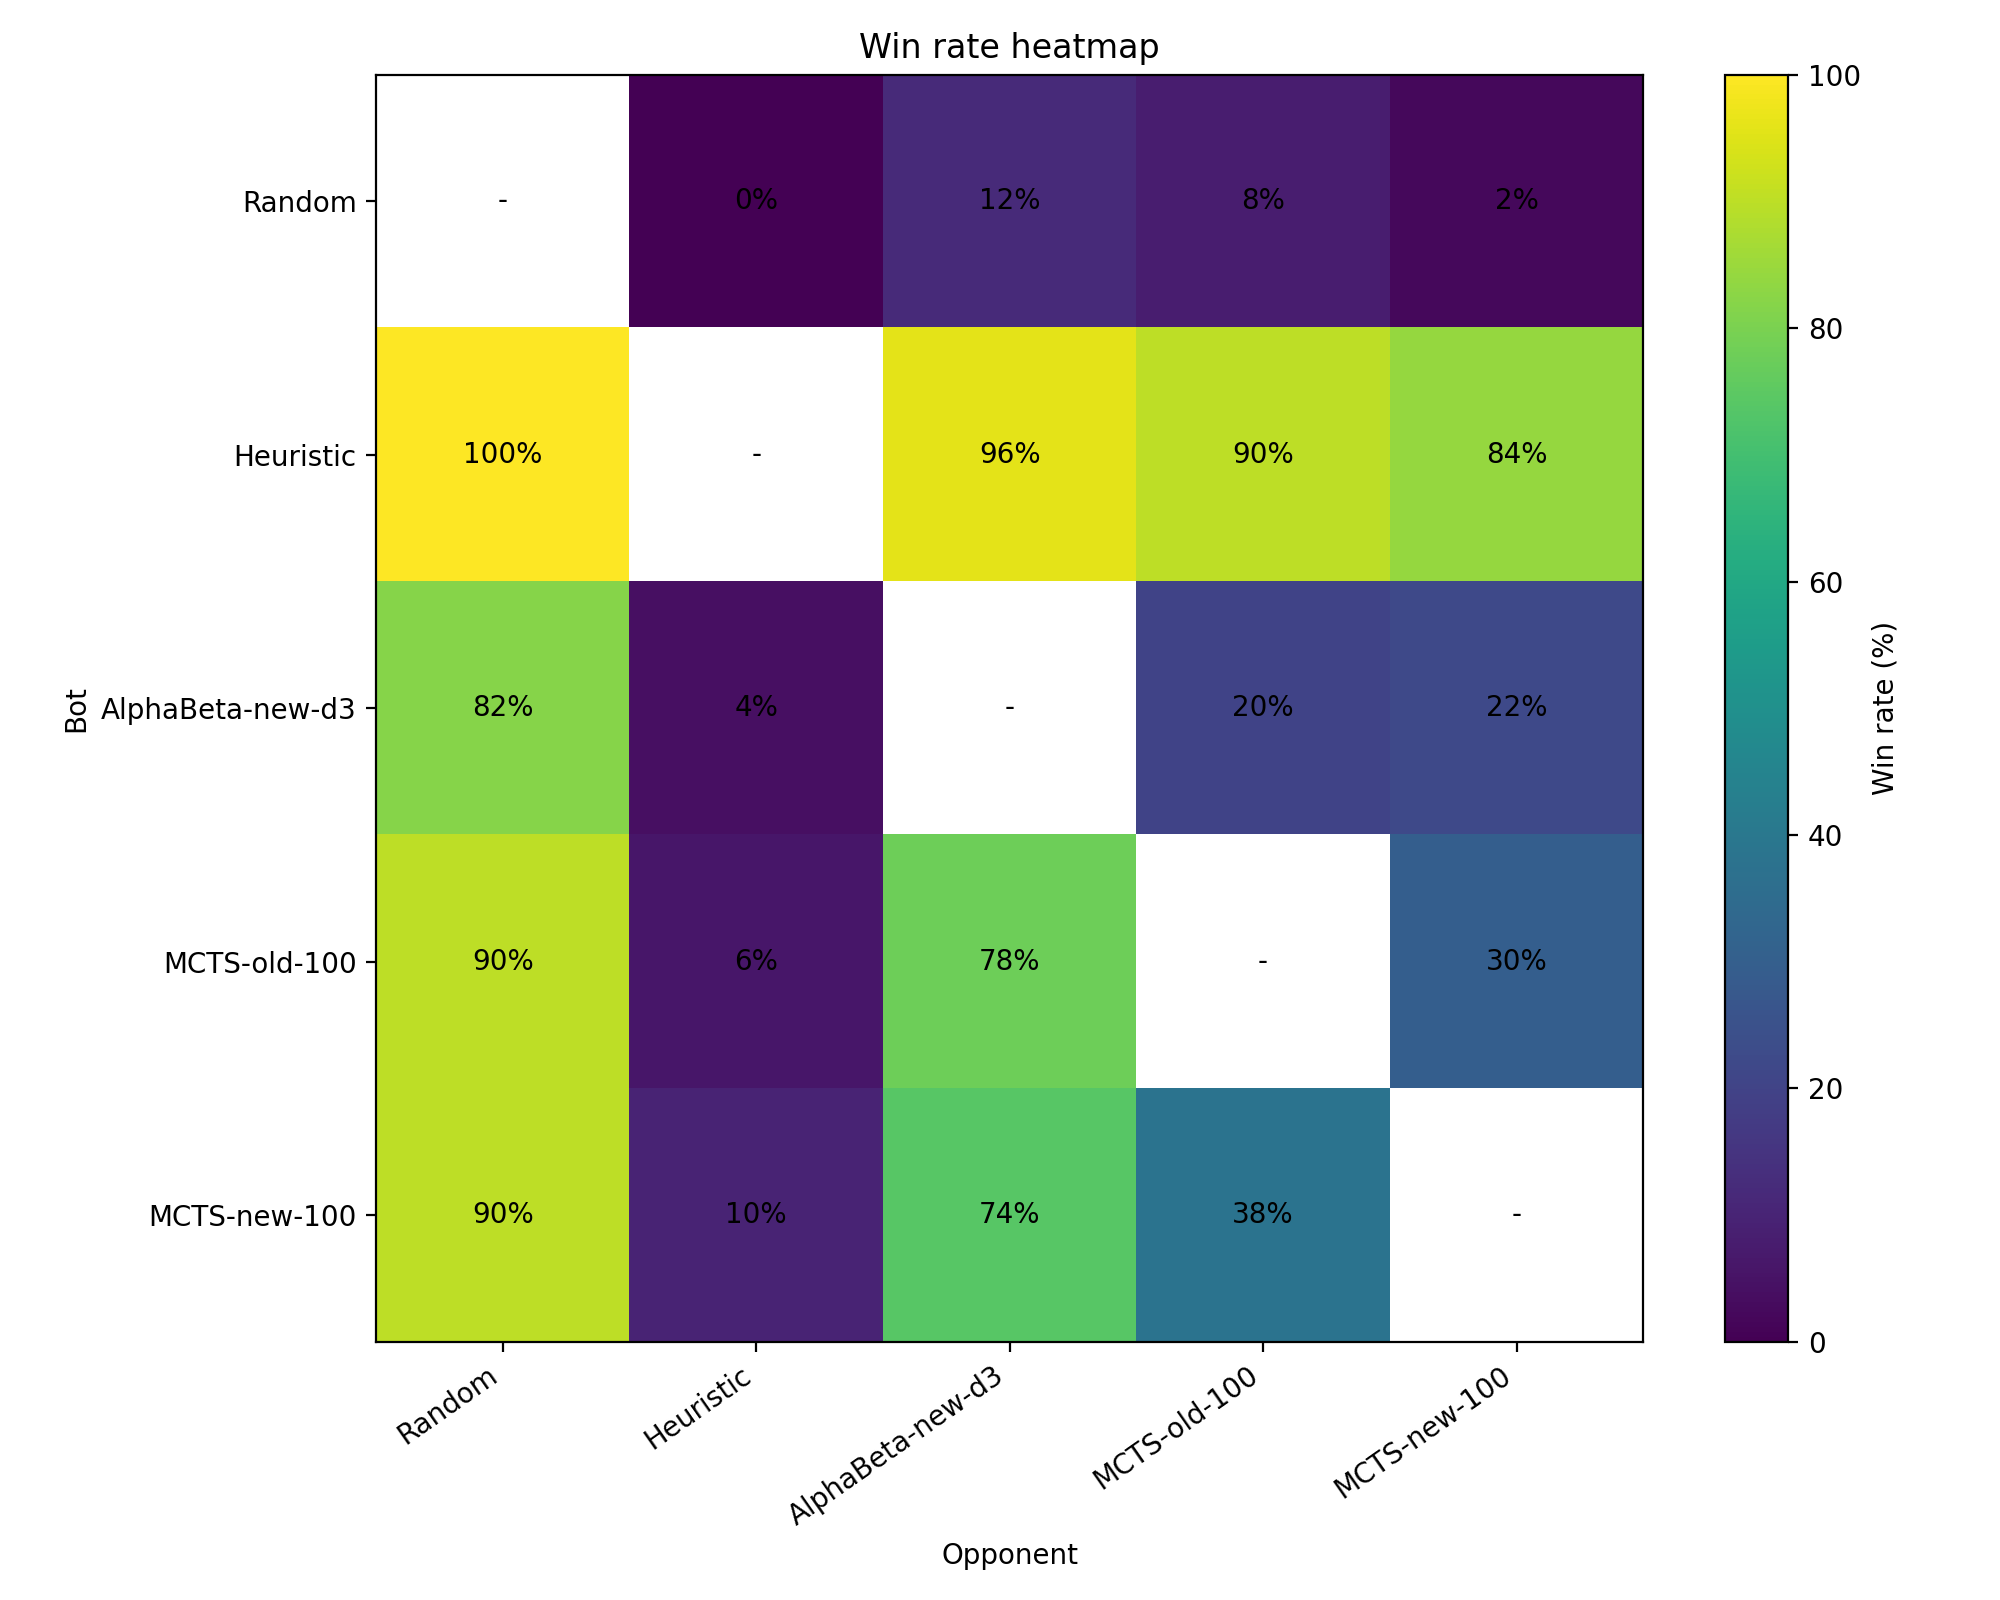
\includegraphics[width=0.99\textwidth]{img/winrate_heatmap.png}
    \caption{Procento vítězství mezi jednotlivými agenty}
    \label{fig:heatmap}
\end{figure}

Z výsledků lze vidět, že náhodný agent představuje nejslabší verzi umělého agenta. Naopak heuristický agent dosáhl nejvyšší 
úspěšnosti proti všem ostatním agentům a zvítězil ve všech vzájemných soubojích. Druhám nejelpším agentem byl pak agent
využívající MCTS, jen proti heuristickému agentovi byl celkem neúspěšný. Verze staré a nové ohodnocovací funkce měly 
velmi podobné výsledky, ale novější verze o nšco lepší. Nejhorším z uměle inteligentních agentů byl agent využívající
minimax a alfa-beta ořezávání.

Celkové bodové hodnocení agentů je znázorněno na obrázku~\ref{fig:tournament_score}.

\begin{figure}[H]
    \centering
    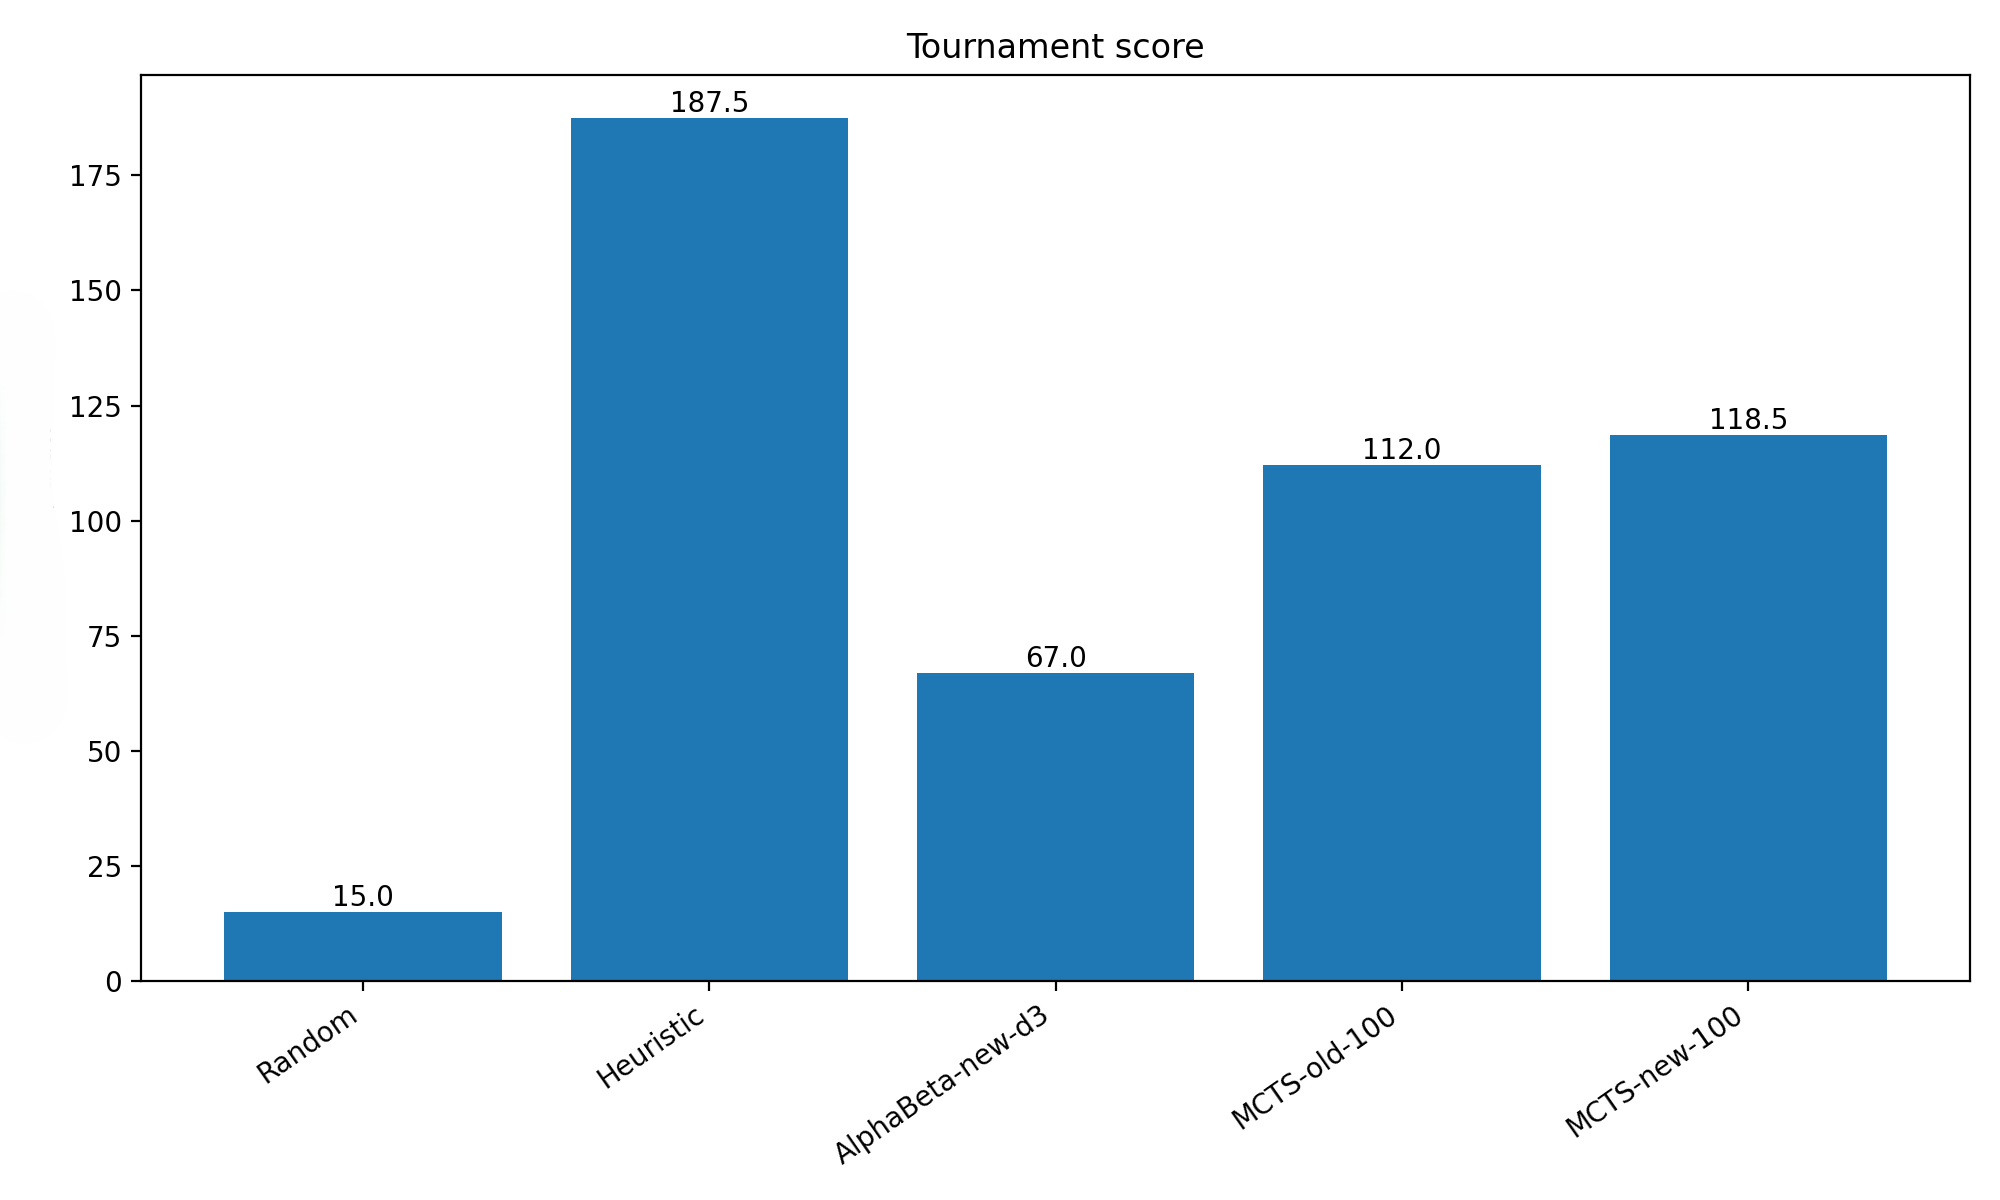
\includegraphics[width=0.99\textwidth]{img/total_scores.png}
    \caption{Celkové skóre agentů.}
    \label{fig:tournament_score}
\end{figure}

Tady je tedy dobře vidět porovnání agentů:

\[
\mathrm{Heuristic} > \mathrm{MCTS}_{\mathrm{new}} > \mathrm{MCTS}_{\mathrm{old}} > \mathrm{AlphaBeta} > \mathrm{Random}
\]

Obrázek~\ref{fig:game_length} porovnává průměrnou délku partií jednotlivých agentů.

\begin{figure}[H]
    \centering
    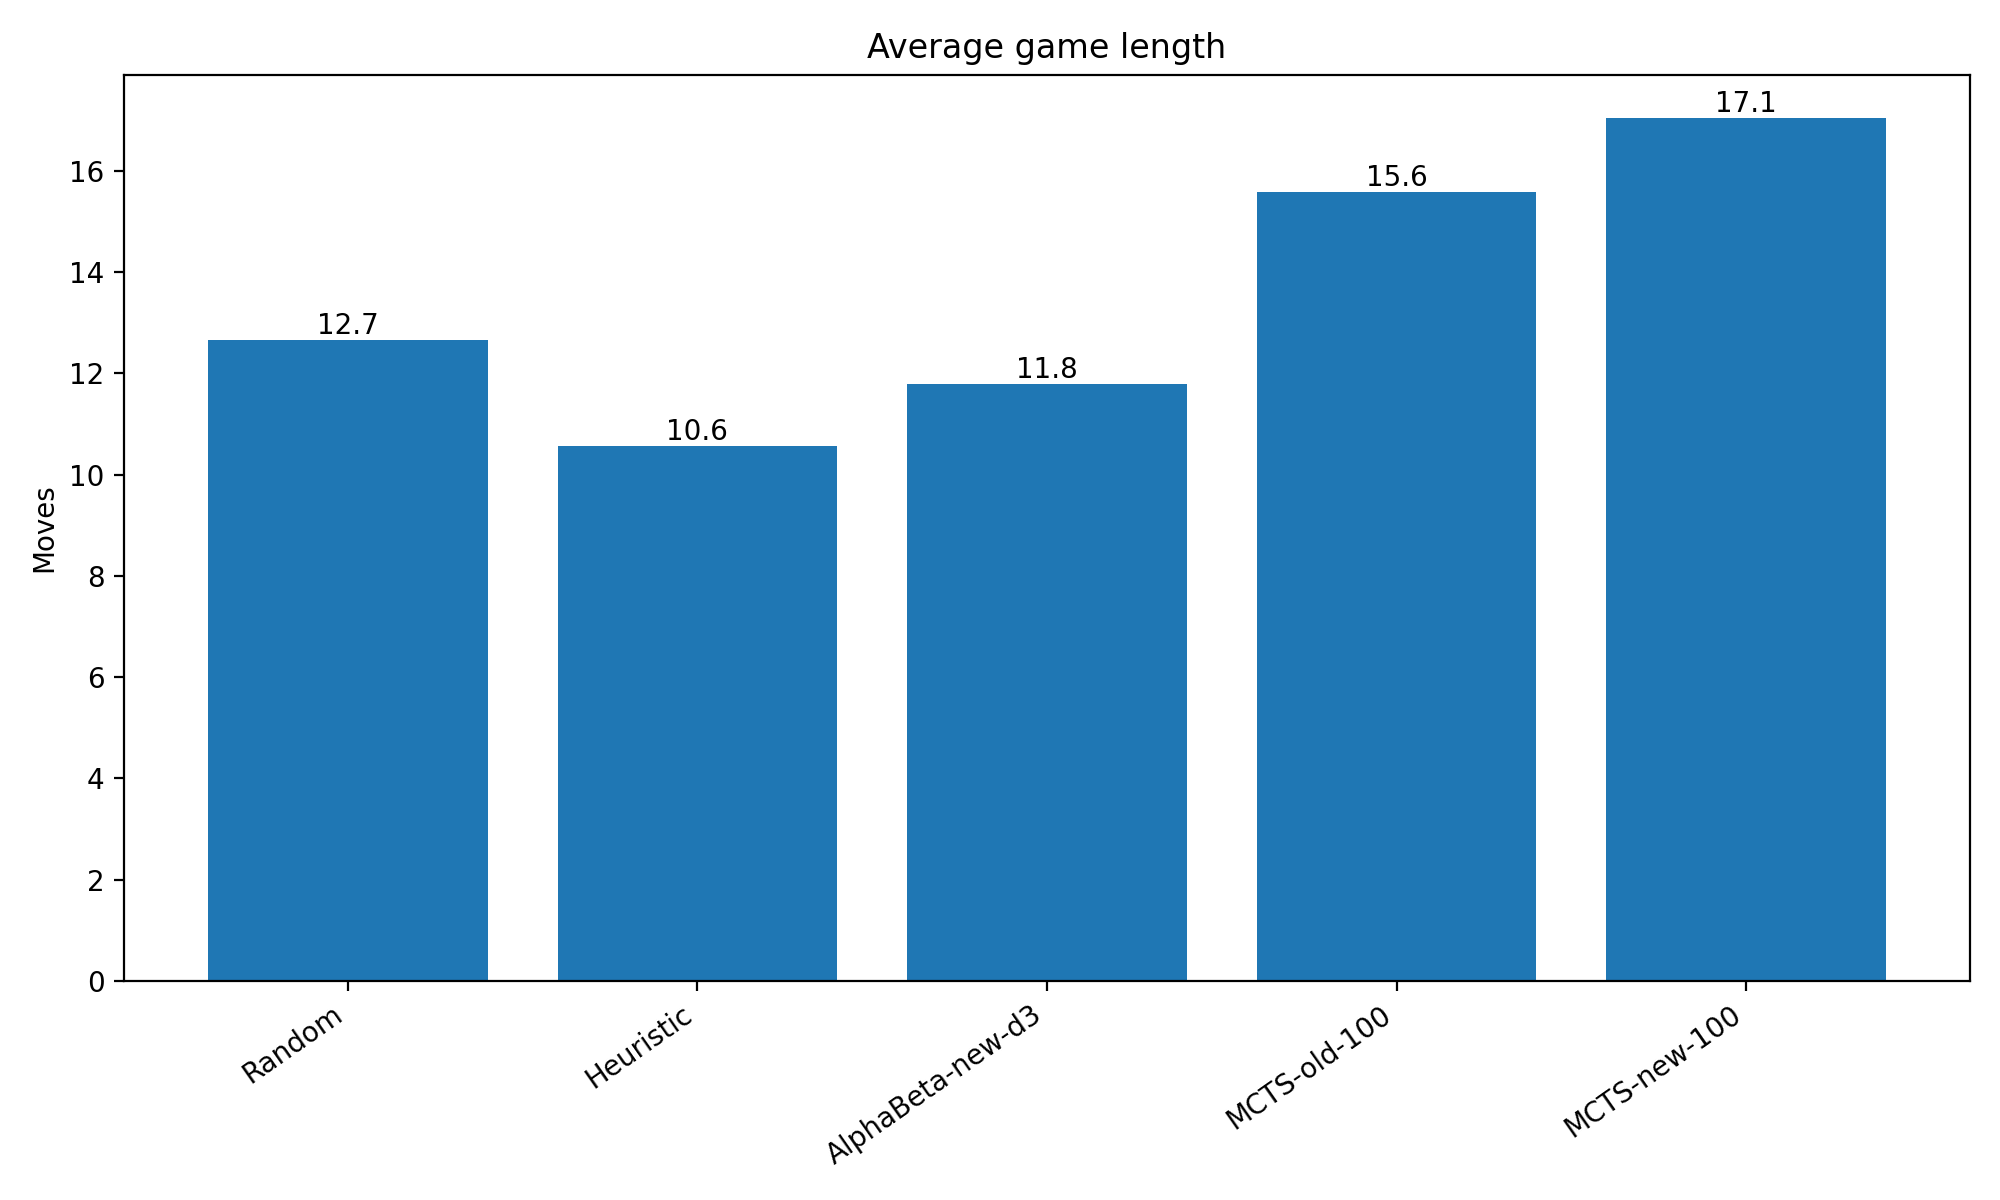
\includegraphics[width=0.99\textwidth]{img/avg_moves.png}
    \caption{Průměrná delka partie agentů.}
    \label{fig:game_length}
\end{figure}

Heuristický agent končí partie nejrychleji, zatímco agent MCTS nejpomaleji.

\subsection{Diskuze}

Přestože se očekávalo, že agent využívající algoritmus MCTS dosáhne nejlepších výsledků, tak experimenty ukázaly odlišné výsledky.
Nejlépe hrál heuristický agent, který hrál velmi podobně lidskému hráči, jelikož jeho heuristika byla navrhnuta subjektivně autorem,
podle jeho mínění o samotné hře. MCTS a alfa-beta boti nedosáhli dobrých výsledků, nejspíš kvůli několika faktorům.
Prvním a tím nejdůležitějším je kvalita neuronové sítě. Oba agenti ji využívají velmi silně a jsou na ní tudíž 
závislí. Nedostatečná kvalita neuronové sítě tedy vede k podprůměrnému chování agenta. Mezi další důvody patří 
nastavené parametry. U těch bylo však přihlíženo k časové efektivitě, tedy více simulací nebo vyšší hloubka prohledávání
už jsou časově přes hranici. Po krátkých testech s jinými hodnotami byly však výsledky podobné, heuristický agent měl stále navrch,
což nás vrací zpět k tomu, že hlavním důvodem bude nedostatečná kvalita sítě.

\section{Vyhodnocení natrénované neuronové sítě}

\subsection{Porovnání s ostatními agenty}

Jak již bylo nastíněno v předešlé diskuzi, natrénovaná neuronová síť byla v algoritmech, které ji využívají, nedostatečná.
Heuristický agent si hravě poradil s těmito agenty, tudíž nedosahuje kvalit, které byly očekávány. Avšak dobrou zprávou je, že 
agenti MCTS i alfa-beta poráželi náhodného agenta, tedy jsou lepší než náhodný výběr. To vede k diskuzi o tom, zda heuristika jednotlivých
agentů nehraje větší roli než samotná neuronová síť. Podle dalších menších testů ale i bez heuristik hráli agenti lépe, než náhodný agent.

\subsection{Diskuze a možnosti dalšího zlepšení}

Dobrou zprávou je, že porovnání agentů algoritmu MCTS s odlišně natrénovanými neuronovými sítěmi ukazuje, že pozdější verze jsou o něco
lepší než starší verze. To vede k myšlence, že další trénování by mohlo neuronovou síť zlepšit. Kromě dalšího trénování u této verze nelze najít
mnoho dalších metod zlepšení.

Druhou variantou by bylo celou neuronovou síť zahodit a její implementaci přehodnotit a jinak implementovat. V této práci byla zvolena jednoduchá
architektura inspirovaná sítí AlphaZero. Odlišná neuronová síť by se mohla zaměřit na lepší konvoluční architekturu, využití reziduálních bloků
nebo jiných modernějších architektur. Současně by mohlo být vhodné změnit reprezentaci herního stavu či jiným způsobem kódovat vstupní data,
což by mohlo síti pomoci zachytit strategické vlastnosti hry.

\section{Porovnání s lidským hráčem}

Cílem tohoto experimentu bylo ověřit, jak si agenti stojí proti lidskému protivníkovi. Zde cílem není získat žádné výsledky, ale spíše zhodnotit 
herní styly samotných agentů.

\subsection{Metodika}

Proti každému agentovi bylo sehráno mezi pěti a deseti hrami. U agentů, u kterách bylo jasné po prvních parttiích, jak se chovají, nebylo více her nutných.

\subsection{Pozorování}

Výsledky jsou podobné jako při turnaji, co se subjektivního ohodnocení týče, ale ani jeden z agentů nedokázal konzistentně vyhrávat.

Náhodný agent, jak bylo očekáváno, byl nejjednoduším protivníkem. Hra většinou konšila před desátým tahem, jelikož se agent nesnaží bránit ani útočit.
Náhodný agent tedy nezaznamenal jediné vítězství.

Alfa-beta agent a agenti využívající MCTS už byli o něco lepší. Partie trvaly kolem 12 tahů. Agenti si lépe hlídali, zda se protivník neblíží vítězství
a zároveň i vlastní tvary tvořili. Na strategie lidského protivníka ale nestačili a vždy se našla výherní cesta, kterou agent nezaznamenal. Ani tito
agenti nezaznamenali jediné vítšzství proti autorovi.

Nejlepším agentem byl heuristický. Ten, jak bylo dříve popsáno, hrál velmi podobně lidskému protivníkovi. Ze zkušeností autora s touto hrou vychází pozorování,
že tahy, které agent provádí, jsou velmi často ty, které by sám udělal. Z deseti sehraných partií autor vyhrál 8. 2 partie, které se botovi podařilo vyhrát,
byly z nepozornosti autora, neboli lidskou chybou.

\section{Shrnutí experimentů}

Experimenty ukázaly funkčnost nacržených agentů a jejich kvalitu. Všichni agenti byli schopní odehrát partii až do konce a jejich výkony bylo možné 
porovnávat pomoí turnaje.

Nejlepších výsledků dosahoval heuristický agent, jehož ručně navržená ohodnocovací funkce se ukázala být pro současnou verzi hry velmi účinná.
Agenti využívající neuronovou síť nebyli schopni heuristického agenta porazit, přesto však měli lepší výsledky, než agent náhodný. Porovnání
různých verzí neuronové sítě navíc ukázalo, že se s časem trénování zlepšuje.

Z výsledků se dá odvodit, že navržená trénovací pipeline je funkční a bylo by ji možné používat jako základ pro další vývoj. Budoucí práce na toto téma
by se měla hlavně zaměřit na kvalitnější architekturu neuronové sítě.